\documentclass[twoside]{book}

% Packages required by doxygen
\usepackage{fixltx2e}
\usepackage{calc}
\usepackage{doxygen}
\usepackage[export]{adjustbox} % also loads graphicx
\usepackage{graphicx}
\usepackage[utf8]{inputenc}
\usepackage{makeidx}
\usepackage{multicol}
\usepackage{multirow}
\PassOptionsToPackage{warn}{textcomp}
\usepackage{textcomp}
\usepackage[nointegrals]{wasysym}
\usepackage[table]{xcolor}

% Font selection
\usepackage[T1]{fontenc}
\usepackage[scaled=.90]{helvet}
\usepackage{courier}
\usepackage{amssymb}
\usepackage{sectsty}
\renewcommand{\familydefault}{\sfdefault}
\allsectionsfont{%
  \fontseries{bc}\selectfont%
  \color{darkgray}%
}
\renewcommand{\DoxyLabelFont}{%
  \fontseries{bc}\selectfont%
  \color{darkgray}%
}
\newcommand{\+}{\discretionary{\mbox{\scriptsize$\hookleftarrow$}}{}{}}

% Page & text layout
\usepackage{geometry}
\geometry{%
  a4paper,%
  top=2.5cm,%
  bottom=2.5cm,%
  left=2.5cm,%
  right=2.5cm%
}
\tolerance=750
\hfuzz=15pt
\hbadness=750
\setlength{\emergencystretch}{15pt}
\setlength{\parindent}{0cm}
\setlength{\parskip}{3ex plus 2ex minus 2ex}
\makeatletter
\renewcommand{\paragraph}{%
  \@startsection{paragraph}{4}{0ex}{-1.0ex}{1.0ex}{%
    \normalfont\normalsize\bfseries\SS@parafont%
  }%
}
\renewcommand{\subparagraph}{%
  \@startsection{subparagraph}{5}{0ex}{-1.0ex}{1.0ex}{%
    \normalfont\normalsize\bfseries\SS@subparafont%
  }%
}
\makeatother

% Headers & footers
\usepackage{fancyhdr}
\pagestyle{fancyplain}
\fancyhead[LE]{\fancyplain{}{\bfseries\thepage}}
\fancyhead[CE]{\fancyplain{}{}}
\fancyhead[RE]{\fancyplain{}{\bfseries\leftmark}}
\fancyhead[LO]{\fancyplain{}{\bfseries\rightmark}}
\fancyhead[CO]{\fancyplain{}{}}
\fancyhead[RO]{\fancyplain{}{\bfseries\thepage}}
\fancyfoot[LE]{\fancyplain{}{}}
\fancyfoot[CE]{\fancyplain{}{}}
\fancyfoot[RE]{\fancyplain{}{\bfseries\scriptsize Generated by Doxygen }}
\fancyfoot[LO]{\fancyplain{}{\bfseries\scriptsize Generated by Doxygen }}
\fancyfoot[CO]{\fancyplain{}{}}
\fancyfoot[RO]{\fancyplain{}{}}
\renewcommand{\footrulewidth}{0.4pt}
\renewcommand{\chaptermark}[1]{%
  \markboth{#1}{}%
}
\renewcommand{\sectionmark}[1]{%
  \markright{\thesection\ #1}%
}

% Indices & bibliography
\usepackage{natbib}
\usepackage[titles]{tocloft}
\setcounter{tocdepth}{3}
\setcounter{secnumdepth}{5}
\makeindex

% Hyperlinks (required, but should be loaded last)
\usepackage{ifpdf}
\ifpdf
  \usepackage[pdftex,pagebackref=true]{hyperref}
\else
  \usepackage[ps2pdf,pagebackref=true]{hyperref}
\fi
\hypersetup{%
  colorlinks=true,%
  linkcolor=blue,%
  citecolor=blue,%
  unicode%
}

% Custom commands
\newcommand{\clearemptydoublepage}{%
  \newpage{\pagestyle{empty}\cleardoublepage}%
}

\usepackage{caption}
\captionsetup{labelsep=space,justification=centering,font={bf},singlelinecheck=off,skip=4pt,position=top}

%===== C O N T E N T S =====

\begin{document}

% Titlepage & ToC
\hypersetup{pageanchor=false,
             bookmarksnumbered=true,
             pdfencoding=unicode
            }
\pagenumbering{alph}
\begin{titlepage}
\vspace*{7cm}
\begin{center}%
{\Large Magma Engine }\\
\vspace*{1cm}
{\large Generated by Doxygen 1.8.13}\\
\end{center}
\end{titlepage}
\clearemptydoublepage
\pagenumbering{roman}
\tableofcontents
\clearemptydoublepage
\pagenumbering{arabic}
\hypersetup{pageanchor=true}

%--- Begin generated contents ---
\chapter{Hierarchical Index}
\section{Class Hierarchy}
This inheritance list is sorted roughly, but not completely, alphabetically\+:\begin{DoxyCompactList}
\item \contentsline{section}{Magma\+:\+:Console}{\pageref{class_magma_1_1_console}}{}
\begin{DoxyCompactList}
\item \contentsline{section}{Magma\+:\+:Null\+Console}{\pageref{class_magma_1_1_null_console}}{}
\end{DoxyCompactList}
\item istream\begin{DoxyCompactList}
\item \contentsline{section}{ifunctionstream}{\pageref{classifunctionstream}}{}
\end{DoxyCompactList}
\item ostream\begin{DoxyCompactList}
\item \contentsline{section}{ofunctionstream}{\pageref{classofunctionstream}}{}
\end{DoxyCompactList}
\item streambuf\begin{DoxyCompactList}
\item \contentsline{section}{ifunctionbuf}{\pageref{classifunctionbuf}}{}
\begin{DoxyCompactList}
\item \contentsline{section}{ifunctionstream}{\pageref{classifunctionstream}}{}
\end{DoxyCompactList}
\item \contentsline{section}{ofunctionbuf}{\pageref{classofunctionbuf}}{}
\begin{DoxyCompactList}
\item \contentsline{section}{ofunctionstream}{\pageref{classofunctionstream}}{}
\end{DoxyCompactList}
\end{DoxyCompactList}
\end{DoxyCompactList}

\chapter{Class Index}
\section{Class List}
Here are the classes, structs, unions and interfaces with brief descriptions\+:\begin{DoxyCompactList}
\item\contentsline{section}{\hyperlink{class_magma_1_1_console}{Magma\+::\+Console} \\*Interface used to create a layer of abstraction between the multiple types of consoles. Default console type is \hyperlink{class_magma_1_1_null_console}{Null\+Console}. }{\pageref{class_magma_1_1_console}}{}
\item\contentsline{section}{\hyperlink{class_magma_1_1_null_console}{Magma\+::\+Null\+Console} \\*Null \hyperlink{class_magma_1_1_console}{Console} implementation }{\pageref{class_magma_1_1_null_console}}{}
\item\contentsline{section}{\hyperlink{class_magma_1_1_s_t_d_console}{Magma\+::\+S\+T\+D\+Console} \\*Standard \hyperlink{class_magma_1_1_console}{Console} implementation (using C++ standard library) }{\pageref{class_magma_1_1_s_t_d_console}}{}
\end{DoxyCompactList}

\chapter{Class Documentation}
\hypertarget{class_magma_1_1_console}{}\section{Magma\+:\+:Console Class Reference}
\label{class_magma_1_1_console}\index{Magma\+::\+Console@{Magma\+::\+Console}}


Interface used to create a layer of abstraction between the multiple types of consoles. Default console type is \hyperlink{class_magma_1_1_null_console}{Null\+Console}.  




{\ttfamily \#include $<$Console.\+hpp$>$}

Inheritance diagram for Magma\+:\+:Console\+:\begin{figure}[H]
\begin{center}
\leavevmode
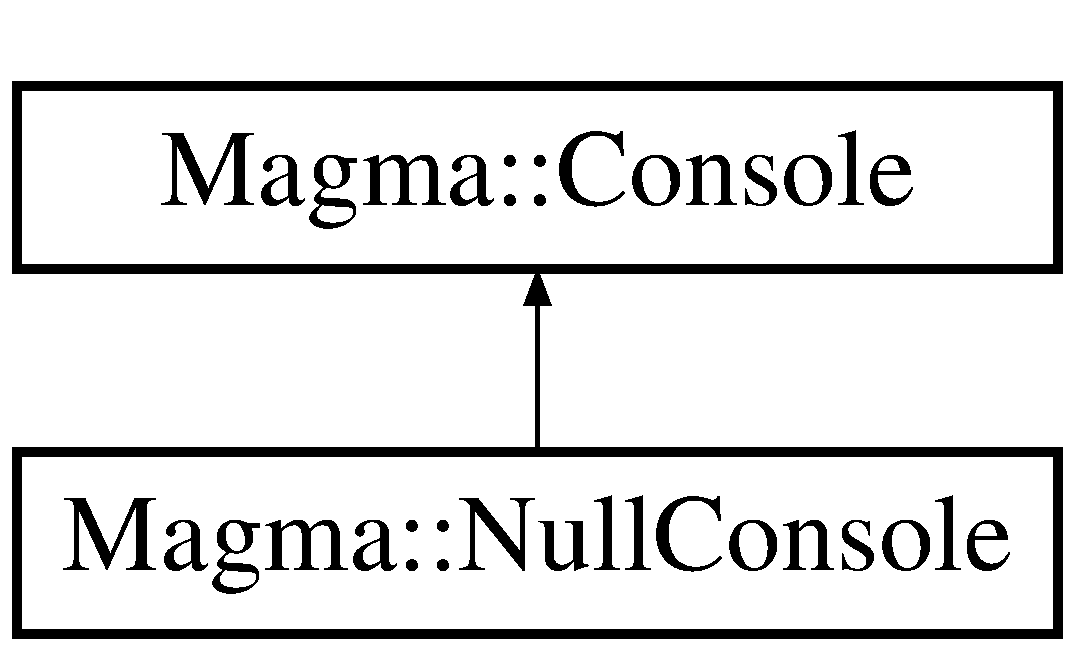
\includegraphics[height=2.000000cm]{class_magma_1_1_console}
\end{center}
\end{figure}
\subsection*{Static Public Member Functions}
\begin{DoxyCompactItemize}
\item 
{\footnotesize template$<$typename T $>$ }\\static void \hyperlink{class_magma_1_1_console_a378572ada79137830c60c52371fcc24e}{Set} ()
\begin{DoxyCompactList}\small\item\em Sets the current console type \end{DoxyCompactList}\item 
static void \hyperlink{class_magma_1_1_console_a86389ac097431a8c5a58b0afa5251a6b}{Print} (const std\+::string \&out)
\begin{DoxyCompactList}\small\item\em Prints something to the console \end{DoxyCompactList}\item 
static void \hyperlink{class_magma_1_1_console_aa8ab1a56c768f05eab042bf76c3447e2}{Print\+Ln} (const std\+::string \&out)
\begin{DoxyCompactList}\small\item\em Prints a whole line to the console \end{DoxyCompactList}\item 
static void \hyperlink{class_magma_1_1_console_afc79ad097b46bfcf38e9bcff89f3354d}{Read} (std\+::string \&in)
\begin{DoxyCompactList}\small\item\em Reads something from the console \end{DoxyCompactList}\item 
static void \hyperlink{class_magma_1_1_console_a984a8294955770ff171817e5e228a629}{Read\+Ln} (std\+::string \&in)
\begin{DoxyCompactList}\small\item\em Reads a whole line from the console \end{DoxyCompactList}\end{DoxyCompactItemize}
\subsection*{Protected Member Functions}
\begin{DoxyCompactItemize}
\item 
\mbox{\Hypertarget{class_magma_1_1_console_a93d5a4745230b85fb5e21c65a4bd1d4f}\label{class_magma_1_1_console_a93d5a4745230b85fb5e21c65a4bd1d4f}} 
virtual void {\bfseries D\+Print} (const std\+::string \&out)=0
\item 
\mbox{\Hypertarget{class_magma_1_1_console_aed105d39eca3a64a54160835206e4a86}\label{class_magma_1_1_console_aed105d39eca3a64a54160835206e4a86}} 
virtual void {\bfseries D\+Print\+Ln} (const std\+::string \&out)=0
\item 
\mbox{\Hypertarget{class_magma_1_1_console_aa36352b1816550648abee51ded18a33f}\label{class_magma_1_1_console_aa36352b1816550648abee51ded18a33f}} 
virtual void {\bfseries D\+Read} (std\+::string \&in)=0
\item 
\mbox{\Hypertarget{class_magma_1_1_console_a6831d8a7f17a0e5a093f5b9ffd3d56bd}\label{class_magma_1_1_console_a6831d8a7f17a0e5a093f5b9ffd3d56bd}} 
virtual void {\bfseries D\+Read\+Ln} (std\+::string \&in)=0
\end{DoxyCompactItemize}


\subsection{Detailed Description}
Interface used to create a layer of abstraction between the multiple types of consoles. Default console type is \hyperlink{class_magma_1_1_null_console}{Null\+Console}. 



\subsection{Member Function Documentation}
\mbox{\Hypertarget{class_magma_1_1_console_a86389ac097431a8c5a58b0afa5251a6b}\label{class_magma_1_1_console_a86389ac097431a8c5a58b0afa5251a6b}} 
\index{Magma\+::\+Console@{Magma\+::\+Console}!Print@{Print}}
\index{Print@{Print}!Magma\+::\+Console@{Magma\+::\+Console}}
\subsubsection{\texorpdfstring{Print()}{Print()}}
{\footnotesize\ttfamily void Magma\+::\+Console\+::\+Print (\begin{DoxyParamCaption}\item[{const std\+::string \&}]{out }\end{DoxyParamCaption})\hspace{0.3cm}{\ttfamily [static]}}



Prints something to the console 


\begin{DoxyParams}{Parameters}
{\em out} & \hyperlink{class_magma_1_1_console}{Console} output string\\
\hline
\end{DoxyParams}
\mbox{\Hypertarget{class_magma_1_1_console_aa8ab1a56c768f05eab042bf76c3447e2}\label{class_magma_1_1_console_aa8ab1a56c768f05eab042bf76c3447e2}} 
\index{Magma\+::\+Console@{Magma\+::\+Console}!Print\+Ln@{Print\+Ln}}
\index{Print\+Ln@{Print\+Ln}!Magma\+::\+Console@{Magma\+::\+Console}}
\subsubsection{\texorpdfstring{Print\+Ln()}{PrintLn()}}
{\footnotesize\ttfamily void Magma\+::\+Console\+::\+Print\+Ln (\begin{DoxyParamCaption}\item[{const std\+::string \&}]{out }\end{DoxyParamCaption})\hspace{0.3cm}{\ttfamily [static]}}



Prints a whole line to the console 


\begin{DoxyParams}{Parameters}
{\em out} & \hyperlink{class_magma_1_1_console}{Console} output string\\
\hline
\end{DoxyParams}
\mbox{\Hypertarget{class_magma_1_1_console_afc79ad097b46bfcf38e9bcff89f3354d}\label{class_magma_1_1_console_afc79ad097b46bfcf38e9bcff89f3354d}} 
\index{Magma\+::\+Console@{Magma\+::\+Console}!Read@{Read}}
\index{Read@{Read}!Magma\+::\+Console@{Magma\+::\+Console}}
\subsubsection{\texorpdfstring{Read()}{Read()}}
{\footnotesize\ttfamily void Magma\+::\+Console\+::\+Read (\begin{DoxyParamCaption}\item[{std\+::string \&}]{in }\end{DoxyParamCaption})\hspace{0.3cm}{\ttfamily [static]}}



Reads something from the console 


\begin{DoxyParams}{Parameters}
{\em in} & \hyperlink{class_magma_1_1_console}{Console} input string\\
\hline
\end{DoxyParams}
\mbox{\Hypertarget{class_magma_1_1_console_a984a8294955770ff171817e5e228a629}\label{class_magma_1_1_console_a984a8294955770ff171817e5e228a629}} 
\index{Magma\+::\+Console@{Magma\+::\+Console}!Read\+Ln@{Read\+Ln}}
\index{Read\+Ln@{Read\+Ln}!Magma\+::\+Console@{Magma\+::\+Console}}
\subsubsection{\texorpdfstring{Read\+Ln()}{ReadLn()}}
{\footnotesize\ttfamily void Magma\+::\+Console\+::\+Read\+Ln (\begin{DoxyParamCaption}\item[{std\+::string \&}]{in }\end{DoxyParamCaption})\hspace{0.3cm}{\ttfamily [static]}}



Reads a whole line from the console 


\begin{DoxyParams}{Parameters}
{\em in} & \hyperlink{class_magma_1_1_console}{Console} input string\\
\hline
\end{DoxyParams}
\mbox{\Hypertarget{class_magma_1_1_console_a378572ada79137830c60c52371fcc24e}\label{class_magma_1_1_console_a378572ada79137830c60c52371fcc24e}} 
\index{Magma\+::\+Console@{Magma\+::\+Console}!Set@{Set}}
\index{Set@{Set}!Magma\+::\+Console@{Magma\+::\+Console}}
\subsubsection{\texorpdfstring{Set()}{Set()}}
{\footnotesize\ttfamily template$<$typename T $>$ \\
void Magma\+::\+Console\+::\+Set (\begin{DoxyParamCaption}{ }\end{DoxyParamCaption})\hspace{0.3cm}{\ttfamily [inline]}, {\ttfamily [static]}}



Sets the current console type 



The documentation for this class was generated from the following files\+:\begin{DoxyCompactItemize}
\item 
src/\+Magma/\+Debug/Console.\+hpp\item 
src/\+Magma/\+Debug/Console.\+cpp\end{DoxyCompactItemize}

\hypertarget{classifunctionbuf}{}\section{ifunctionbuf Class Reference}
\label{classifunctionbuf}\index{ifunctionbuf@{ifunctionbuf}}
Inheritance diagram for ifunctionbuf\+:\begin{figure}[H]
\begin{center}
\leavevmode
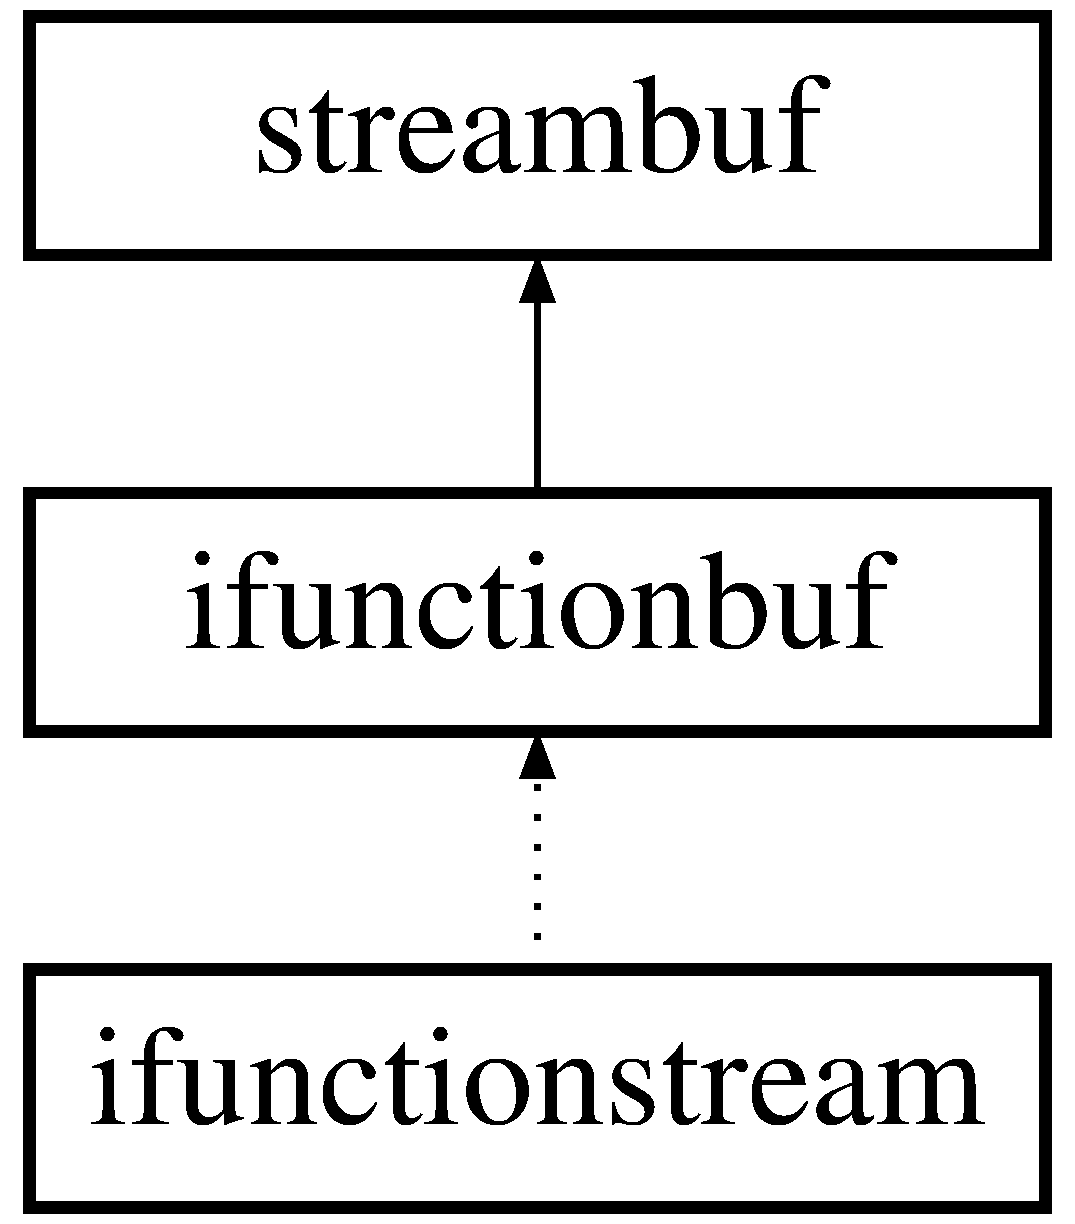
\includegraphics[height=3.000000cm]{classifunctionbuf}
\end{center}
\end{figure}
\subsection*{Public Member Functions}
\begin{DoxyCompactItemize}
\item 
\mbox{\Hypertarget{classifunctionbuf_a6e068a70a5044221e7b3f53b969e02a5}\label{classifunctionbuf_a6e068a70a5044221e7b3f53b969e02a5}} 
{\bfseries ifunctionbuf} (std\+::function$<$ void(std\+::string \&)$>$ const \&function)
\end{DoxyCompactItemize}


The documentation for this class was generated from the following file\+:\begin{DoxyCompactItemize}
\item 
D\+:/\+Programação/\+Ricardo/\+Magma-\/\+Engine/\+Solution/\+Magma/src/\+Magma/\+Debug/Console.\+cpp\end{DoxyCompactItemize}

\hypertarget{classifunctionstream}{}\section{ifunctionstream Class Reference}
\label{classifunctionstream}\index{ifunctionstream@{ifunctionstream}}
Inheritance diagram for ifunctionstream\+:\begin{figure}[H]
\begin{center}
\leavevmode
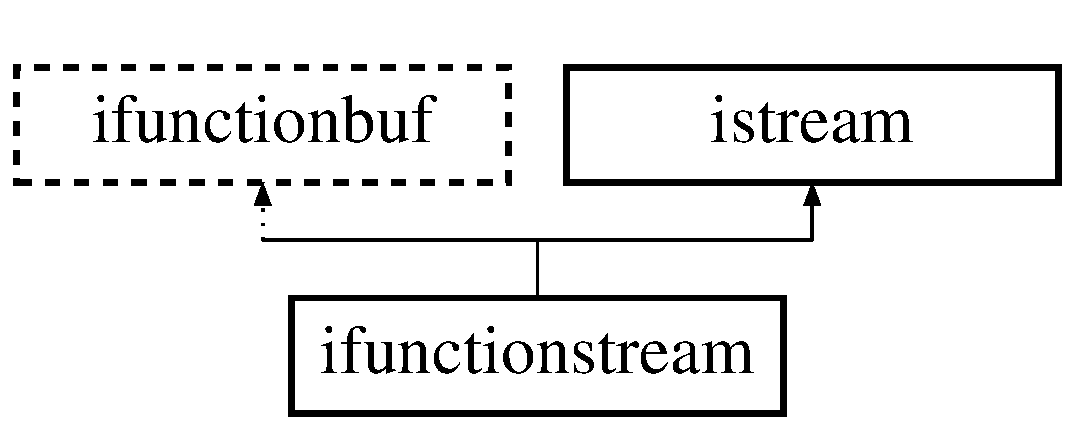
\includegraphics[height=2.000000cm]{classifunctionstream}
\end{center}
\end{figure}
\subsection*{Public Member Functions}
\begin{DoxyCompactItemize}
\item 
\mbox{\Hypertarget{classifunctionstream_ac41a505da4c3feef9bf26692dda6728e}\label{classifunctionstream_ac41a505da4c3feef9bf26692dda6728e}} 
{\bfseries ifunctionstream} (std\+::function$<$ void(std\+::string \&)$>$ const \&function)
\end{DoxyCompactItemize}


The documentation for this class was generated from the following file\+:\begin{DoxyCompactItemize}
\item 
D\+:/\+Programação/\+Ricardo/\+Magma-\/\+Engine/\+Solution/\+Magma/src/\+Magma/\+Debug/Console.\+cpp\end{DoxyCompactItemize}

\hypertarget{class_magma_1_1_null_console}{}\section{Magma\+:\+:Null\+Console Class Reference}
\label{class_magma_1_1_null_console}\index{Magma\+::\+Null\+Console@{Magma\+::\+Null\+Console}}


Null implementation of \hyperlink{class_magma_1_1_console}{Console} interface  




{\ttfamily \#include $<$Console.\+hpp$>$}

Inheritance diagram for Magma\+:\+:Null\+Console\+:\begin{figure}[H]
\begin{center}
\leavevmode
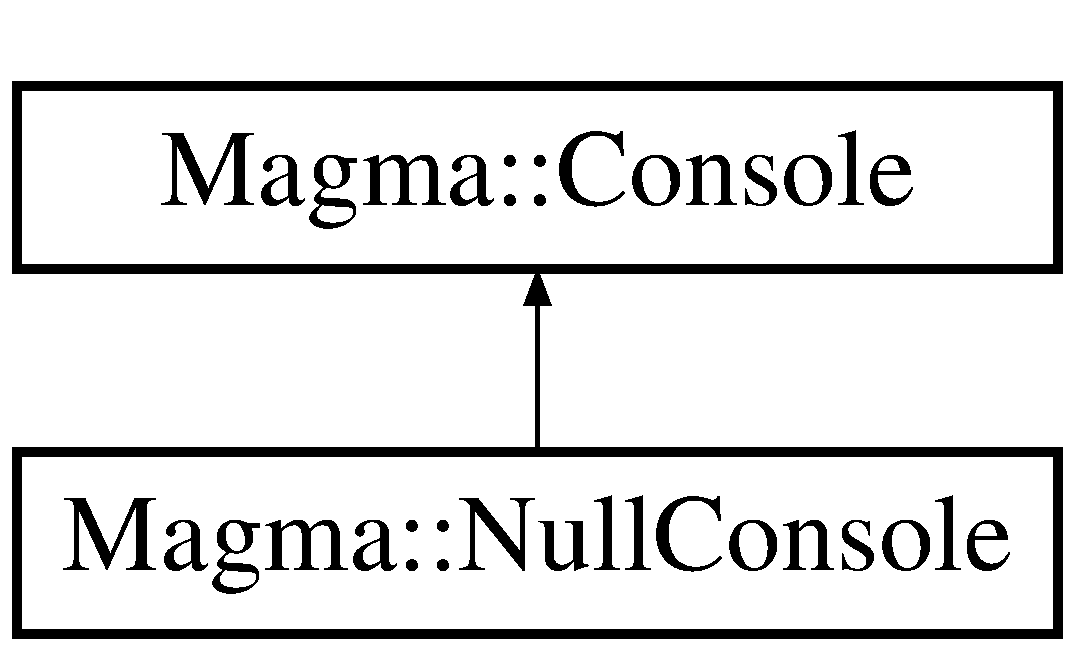
\includegraphics[height=2.000000cm]{class_magma_1_1_null_console}
\end{center}
\end{figure}
\subsection*{Public Member Functions}
\begin{DoxyCompactItemize}
\item 
\mbox{\Hypertarget{class_magma_1_1_null_console_a0ede89f63242d86719b73dbf19fb2fdb}\label{class_magma_1_1_null_console_a0ede89f63242d86719b73dbf19fb2fdb}} 
virtual void {\bfseries D\+Print} (const std\+::string \&text) final
\item 
\mbox{\Hypertarget{class_magma_1_1_null_console_a673f778c29304e00fe095946a830f5f2}\label{class_magma_1_1_null_console_a673f778c29304e00fe095946a830f5f2}} 
virtual void {\bfseries D\+Print\+Ln} (const std\+::string \&text) final
\item 
\mbox{\Hypertarget{class_magma_1_1_null_console_a4d514efc9382dd835bd04e479f545f44}\label{class_magma_1_1_null_console_a4d514efc9382dd835bd04e479f545f44}} 
virtual void {\bfseries D\+Error} (const std\+::string \&text) final
\item 
\mbox{\Hypertarget{class_magma_1_1_null_console_aa6995f1e59cce164ffbebe4c217fe652}\label{class_magma_1_1_null_console_aa6995f1e59cce164ffbebe4c217fe652}} 
virtual void {\bfseries D\+Clear} () final
\end{DoxyCompactItemize}
\subsection*{Additional Inherited Members}


\subsection{Detailed Description}
Null implementation of \hyperlink{class_magma_1_1_console}{Console} interface 



The documentation for this class was generated from the following files\+:\begin{DoxyCompactItemize}
\item 
D\+:/\+Programação/\+Ricardo/\+Magma-\/\+Engine/\+Solution/\+Magma/src/\+Magma/\+Debug/Console.\+hpp\item 
D\+:/\+Programação/\+Ricardo/\+Magma-\/\+Engine/\+Solution/\+Magma/src/\+Magma/\+Debug/Windows\+Console.\+cpp\end{DoxyCompactItemize}

\hypertarget{classofunctionbuf}{}\section{ofunctionbuf Class Reference}
\label{classofunctionbuf}\index{ofunctionbuf@{ofunctionbuf}}
Inheritance diagram for ofunctionbuf\+:\begin{figure}[H]
\begin{center}
\leavevmode
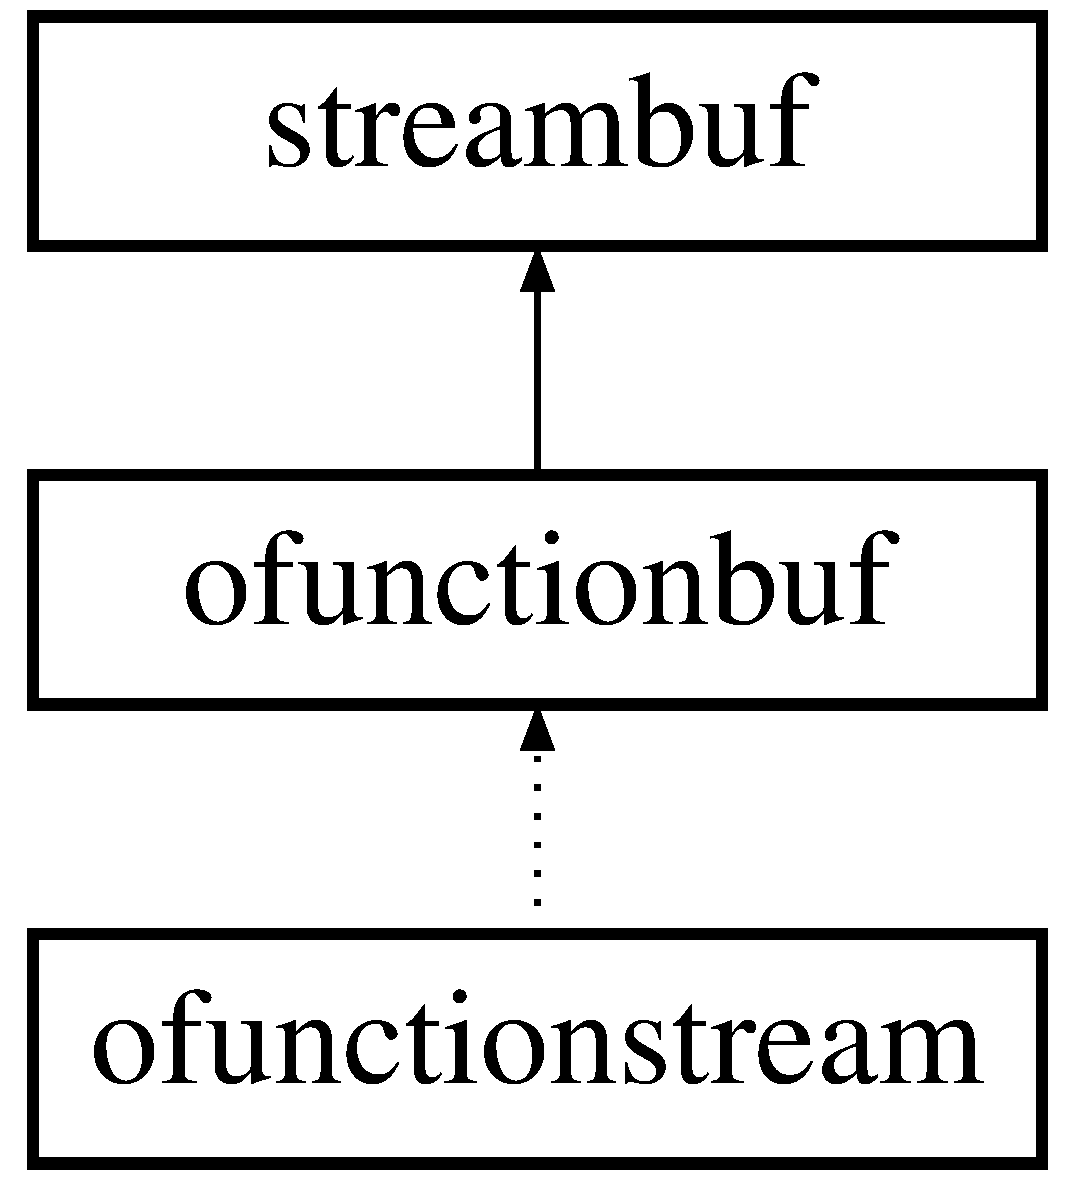
\includegraphics[height=3.000000cm]{classofunctionbuf}
\end{center}
\end{figure}
\subsection*{Public Member Functions}
\begin{DoxyCompactItemize}
\item 
\mbox{\Hypertarget{classofunctionbuf_ac4c827b2738de8c625a1316e15643f3d}\label{classofunctionbuf_ac4c827b2738de8c625a1316e15643f3d}} 
{\bfseries ofunctionbuf} (std\+::function$<$ void(const std\+::string \&)$>$ const \&function)
\end{DoxyCompactItemize}


The documentation for this class was generated from the following file\+:\begin{DoxyCompactItemize}
\item 
src/\+Magma/\+Debug/Console.\+cpp\end{DoxyCompactItemize}

\hypertarget{classofunctionstream}{}\section{ofunctionstream Class Reference}
\label{classofunctionstream}\index{ofunctionstream@{ofunctionstream}}
Inheritance diagram for ofunctionstream\+:\begin{figure}[H]
\begin{center}
\leavevmode
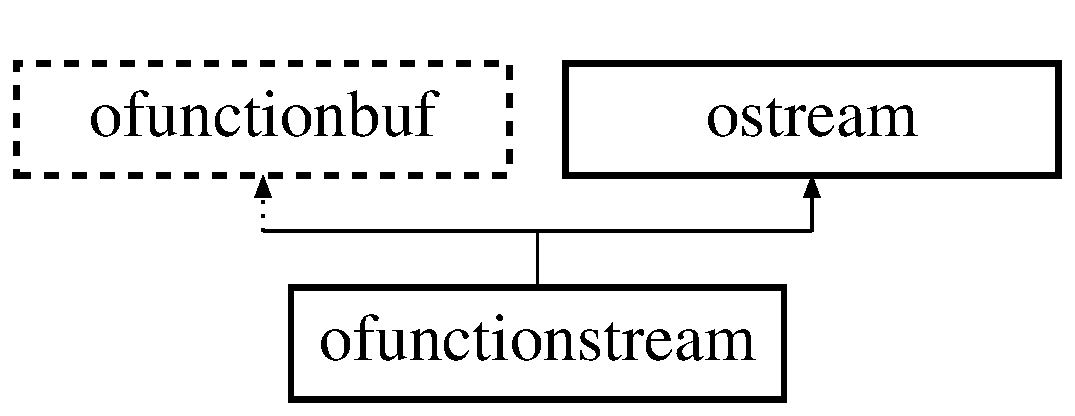
\includegraphics[height=2.000000cm]{classofunctionstream}
\end{center}
\end{figure}
\subsection*{Public Member Functions}
\begin{DoxyCompactItemize}
\item 
\mbox{\Hypertarget{classofunctionstream_a155ec3c7c07fe88d9bd0fe6beb20718f}\label{classofunctionstream_a155ec3c7c07fe88d9bd0fe6beb20718f}} 
{\bfseries ofunctionstream} (std\+::function$<$ void(const std\+::string \&)$>$ const \&function)
\end{DoxyCompactItemize}


The documentation for this class was generated from the following file\+:\begin{DoxyCompactItemize}
\item 
D\+:/\+Programação/\+Ricardo/\+Magma-\/\+Engine/\+Solution/\+Magma/src/\+Magma/\+Debug/Console.\+cpp\end{DoxyCompactItemize}

%--- End generated contents ---

% Index
\backmatter
\newpage
\phantomsection
\clearemptydoublepage
\addcontentsline{toc}{chapter}{Index}
\printindex

\end{document}
